%==================================================================================================
%   LUKES THESIS TEMPLATE 1.2
%   -------------------------
%   This template is based upon the offcial IMM PhD Thesis template, it is enhanced with a number
%   of new features and a number of errors have fixed. This template is intended to be complied to
%   PDF using PDFLATEX and is tested using the MiKTeX 2.9 LaTeX distribution.
%   It is based on the official DTU-IMM Thesis template by Finn Kuno Christensen in 2009.
%   Small bugfixes by Kasper Laursen in 2012 and 2013.
%   Small updates by Finn Kuno Christensen/Henning Christiansen in 2015.
%   -------------------------
%   Last Updated: 2015-01-08
%==================================================================================================
%
%==================================================================================================
% DOCUMENT SETUP
%==================================================================================================
\documentclass[10pt,twoside]{book}                  %Official DTU-IMM Thesis document setup
%
%Set to 'print' for printed version, use 'net' for online version
\def\thesisversion{print}
\providecommand{\master}{.}
%
%==================================================================================================
% PACKAGES
%==================================================================================================

\usepackage{\master/LukeThesis}                             %Import Thesis base style
\usepackage{subfiles}
\usepackage{algorithm}
\usepackage[noend]{algpseudocode}
\usepackage{subcaption}
\usepackage{enumitem}
\usepackage{cleveref}
\usepackage{wasysym}

\usepackage{tikz}
\usetikzlibrary{topaths,calc}
\usetikzlibrary{positioning}
\usetikzlibrary{trees,arrows,fit,shapes}
\usepackage{listings}
\usepackage{xspace}

\lstset{%
	basicstyle=\itshape,
	literate={->}{$\colon =$}{2}
	{α}{$\alpha$}{1}
	{δ}{$\delta$}{1}
	{and}{$\land$}{1}
	{not}{$\neg$}{1}
}

%
%==================================================================================================
% THESIS PROPERTIES (Modifiy these fields with your details)
%==================================================================================================
\def\thesisauthor{Søren Jacobsen and Jannick Johnsen}                     %Author
\def\thesistitle{Action Learning in Automated Planning}               %Title
\def\thesishandin{26-July}                       %Submission date (Day-Month}
\def\thesisdegree{M.Sc.}                              %Degree ('B.Eng', 'B.Sc.', 'M.Sc.' or 'PhD')
\def\thesisyear{2015}                               %Submission year
\def\thesisnumber{????}                             %DTU-IMM Serial number (do not include year)
\def\thesisISSN{0000-0000}                          %ISSN number
\def\thesiskeywords{Keywords are, comma separated}  %PDF keywords
\derivethesisprops                                  %Derive dependent properties
%
%==================================================================================================
% SECTION NUMBERING SETUP
%==================================================================================================
\setcounter{tocdepth}{2}                            %2 adds sections up to subsections
\setcounter{secnumdepth}{3}                         %Subsubsections get a number when this is 3
%
%==================================================================================================
% THESIS STRUCTURE  (Modifiy to include more chapters etc)
%==================================================================================================

% \newtheorem{invariant}{Invariant}[chapter]

\newtheorem{arestriction}{Restriction}  
\theoremstyle{definition}
\newtheorem{definition}{Definition}[chapter]
\theoremstyle{plain}
\newtheorem{example}{Example}[section]
\newtheorem{theorem}{Theorem}[chapter]
\newtheorem{proposition}{Proposition}[chapter]
\newtheorem{invariant}{Invariant}[chapter]
\newtheorem{lemma}{Lemma}[chapter]

\newcommand{\figref}[1]{\figurename~\ref{#1}}

% symbol used for function calculating total state
\newcommand{\ts}{X}


% Symbol for a predicate connection
\newcommand{\pc}{\ensuremath{\times}\xspace}
% Symbol for a binding connection
\newcommand{\bc}{\ensuremath{\ocircle}\xspace}

\newcommand{\rsc}{\ensuremath{\otimes}\xspace}
% Symbol for atoms
\newcommand{\atoms}{\ensuremath{\mathbb{A}}\xspace}

\newcommand{\lits}{\ensuremath{\mathbb{L}}\xspace}
% Symbol for predicates
\newcommand{\preds}{\ensuremath{\mathbb{P}}\xspace}
% Symbol for goal
\newcommand{\goal}{\ensuremath{\mathcal{G}}\xspace}
% Symbol for domain
\newcommand{\dom}{\ensuremath{\mathcal{D}}\xspace}

% symbol for disproven
\newcommand{\dsp}{\ensuremath{d}\xspace}
\newcommand{\Dsp}{\ensuremath{D}\xspace}

% symbol for proven
\newcommand{\pro}{\ensuremath{k}\xspace}
\newcommand{\Pro}{\ensuremath{K}\xspace}

% symbbol for unproven
\newcommand{\up}{\ensuremath{u}\xspace}
\newcommand{\Up}{\ensuremath{U}\xspace}

% symbol for candidate
\newcommand{\cand}{\ensuremath{c}\xspace}
\newcommand{\Cand}{\ensuremath{C}\xspace}

\newcommand{\objs}{\ensuremath{\mathcal{O}}\xspace}

\newcommand{\cset}{\ensuremath{\mathcal{C}}\xspace}

\newcommand{\ground}{\ensuremath{\textit{ground}}\xspace}

\newcommand{\invground}{\ensuremath{\ground ^{-1}}\xspace}

\newcommand{\glits}{\ensuremath{\mathbb{G}}\xspace} 

% Symbol for a conditional
\newcommand{\cond}{\ensuremath{E^C}\xspace}

% symbol for Undefined set
\newcommand{\undefset}{\ensuremath{\mathcal{X}}\xspace}

% symbol for effect set
\newcommand{\geffects}{\ensuremath{\Delta S}\xspace}

% symbol for variables of a conditional
\newcommand{\varC}{\ensuremath{\textit{vars}}\xspace}

% 
\newcommand{\eff}{\ensuremath{\textit{eff}}\xspace}

\newcommand{\pre}{\ensuremath{\textit{pre}}\xspace}

% Font used for Action, Pre, and Eff keywords in schemas
\newcommand{\actt}[1]{\textsc{#1}}
\newcommand{\actpre}{\actt{Pre: }}
\newcommand{\acteff}{\actt{Eff: }}
\newcommand{\actact}{\actt{Action }}

\newcommand{\locref}[1]{\protect\ifthenelse{\pageref{#1}=\thepage}{}{\protect\ifthenelse{\pageref{#1}<\thepage}{, above}{, below}}}

%\let\Cref\locref
\let\oldcref\Cref
\renewcommand{\Cref}[1]{[\oldcref{#1}\locref{#1}]\xspace}

\newcommand{\Sref}[2]{[#1~\ref{#2}\locref{#2}]\xspace}
%\renewcommand{\Cref}[1]{\locref{#1}}
% \let\oldtheorem\theorem
% \renewcommand{\theorem}{%
% 	\crefalias{lemma}{theorem}
% 	\oldtheorem}
%
% \let\oldtheorem\definition
% \renewcommand{\definition}{%
% 	\crefalias{lemma}{definition}
% 	\oldtheorem}
%
% \let\oldtheorem\corollary
% \renewcommand{\corollary}{%
% 	\crefalias{lemma}{corollary}
% 	\oldtheorem}
%
% \let\oldtheorem\proposition
% \renewcommand{\proposition}{%
% 	\crefalias{lemma}{proposition}
% 	\oldtheorem}



\begin{document}

%------------------------
%Pre-frontmatter material
%------------------------
\prefrontmatter
%--------------------
%Frontmatter material
%--------------------
\frontmatter
\pagenumbering{roman}     
\chapter{Abstract}
 
 Action schema learning is important as it is the first step for the construction of an A.I. based on only logical reasoning. 

This thesis deals with action schema learning through deductive reasoning methods.
The purpose of this thesis is show how we may approach Artificial Intelligence learning from non-probabilistic point of view. 
We accomplish this using established mathematical models, such as graphs and sets. 
What the thesis provides is algorithms, mathematical formulas/models for learning STRIPS-style action schema, and gives an insight on how to apply those ideas in conditional-effect action schema learning.



                          %Set frontmatter numbering style
\chapter{Summary (English)}


This thesis attempts to solve the problem of action schema learning.
That is, learning actions in a domain without knowledge of those actions' effects and precondition, and only by analyzing the state-transitions. The solution to these problems should not use any probability or evolutionary theories, but rather infer the actions, based only on analyzing the state-transitions. 
This thesis extends the work of \cite{Walsh2008},
by exploring the underlying properties of their work.
Because of this we are able to remove some of the restrictions in their model.

The goal of this thesis is to elucidate what it means to learn. Specifically we will focus on non-conditional actions, and attempt to provide a framework to solve the problem of conditional action schema learning.

We solve these problems using graph theory, set theory and logic reasoning.

                                   %English summary of Thesis
\markboth{}{}                                       %Set headings (left)(right)
\chapter{Summary (Danish)}
\begin{otherlanguage}{danish}

Denne afhandling forsøger at løse problemerne med at lære actions i et domæne uden kendskab til disse actions' effekter og forudsætninger. Løsningen som vi frembringer er ikke baseret på sandsynlighed eller evolutionære teorier, men snarere at man udleder actions udelukkende baseret på analyse af forskelle mellem konfigurationer af universet.
Denne afhandling udvider arbejdet i~\cite{Walsh2008},
ved at udforske de underliggende egenskaber af deres arbejde.
På grund af dette er vi i stand til at fjerne nogle begrænsninger i deres model.

Målet med denne afhandling er at belyse hvad det betyder at lære. Specielt vil vi fokusere på non-conditional actions, og forsøger at skabe en ramme for at løse problemet med conditional action schema læring.

Vi løser disse problemer ved hjælp af graf-teori, mængde-teori og logisk ræsonnement.

\end{otherlanguage}
                                   %Danish summary of Thesis
\markboth{}{}                                       %Set headings (left)(right)
\chapter{Preface}

This thesis was prepared at DTU Compute in fulfilment of the requirements for acquiring an M.Sc. in Engineering.

This thesis focus on non-conditional and conditional action schema learning.
It extends the work of \cite{Walsh2008}, but also uses ideas from the scientific method which has evolved through many greek philosophers, and we have been heavily inspired by the works of \cite{popper1959a}.

This thesis will provide a proposal about a general agent learning algorithm, a complete a analysis of non-conditional action learning; and a framework and framing of the problems with conditional action learning, and provide initial proposals a solution.
%==================================================================================================
% SIGNATURE AREA
%==================================================================================================
\vspace{20mm}
\begin{center}
    \hspace{20mm} Lyngby, \thesishandin-\thesisyear
    \vspace{5mm}
    \newline
  %Update signature image file in line below
    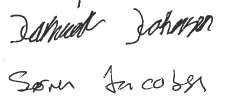
\includegraphics[scale=0.8]{Graphics/signatures}
\end{center}
\begin{flushright}
    \thesisauthor
\end{flushright}
% % % EOF % % %
                                     %Preface
\markboth{}{}                                       %Set headings (left)(right)
\chapter{Acknowledgements}

I would like to thank my....

                            %Acknowledgements
\markboth{}{}                                       %Set headings (left)(right)
%------------------
% Table of contents
%------------------
\newpage\mbox{}\newpage
\chaptermark{Contents}
\pdfbookmark{\contentsname}{toc}
\renewcommand{\sectionmark}[1]{\markright{#1}}
\sectionmark{Contents}
\addtolength{\parskip}{-\baselineskip}
\tableofcontents
\listofalgorithms
\addtolength{\parskip}{\baselineskip}
\renewcommand{\sectionmark}[1]{\markright{\thesection\ #1}}

%-------------
% Main content
%-------------
\mainmatter
\chapter{Introduction}
	\subfile{Introduction}

\chapter{Overview of Learning} \label{sec:Learning}
    \subfile{Learning}

\chapter{Proposal: Generalized algorithm for learning}\label{sec:Algorithm}
	\subfile{Learning/Algorithm}
	\section{Example: PDDL-specific algorithm}\label{sec:PDDLAlgo}
	\subfile{Learning/PDDLAlgorithm}

\chapter{Analysis: Non-conditional actions} \label{chp:nca}
    \subfile{NonConditional}

\chapter{Analysis: Conditional actions}\label{chp:ca}
    \subfile{Conditional}

\chapter{Proof of concept: Simulation}\label{chp:imp}
    \subfile{Implementation}

\chapter{Discussion}\label{chp:dis}
    \subfile{Discussion}

\chapter{Conclusion}
	\subfile{Conclusion}

\appendix
\chapter{PDDL}\label{sec:app:pddl}
    \subfile{Appendices/PDDL}
\chapter{Conditional learning with hypergraphs}\label{sec:app:hypergraph}
    \subfile{Appendices/Hypergraph}
\chapter{Results}\label{sec:app:results}
    \subfile{Appendices/Results}
%-----------
% Backmatter
%-----------
\backmatter
\chaptermark{Bibliography}
\renewcommand{\sectionmark}[1]{\markright{#1}}
\sectionmark{Bibliography}
\addcontentsline{toc}{chapter}{Bibliography}        %Force addition of Bibliography to TOC
\bibliographystyle{alpha}                           %Use alpha codes for references
\bibliography{refs}                           %Bibliography file called
\end{document}
% % % EOF % % %
